\section{Architecture Overview}

\begin{figure}[H]
    \centering
    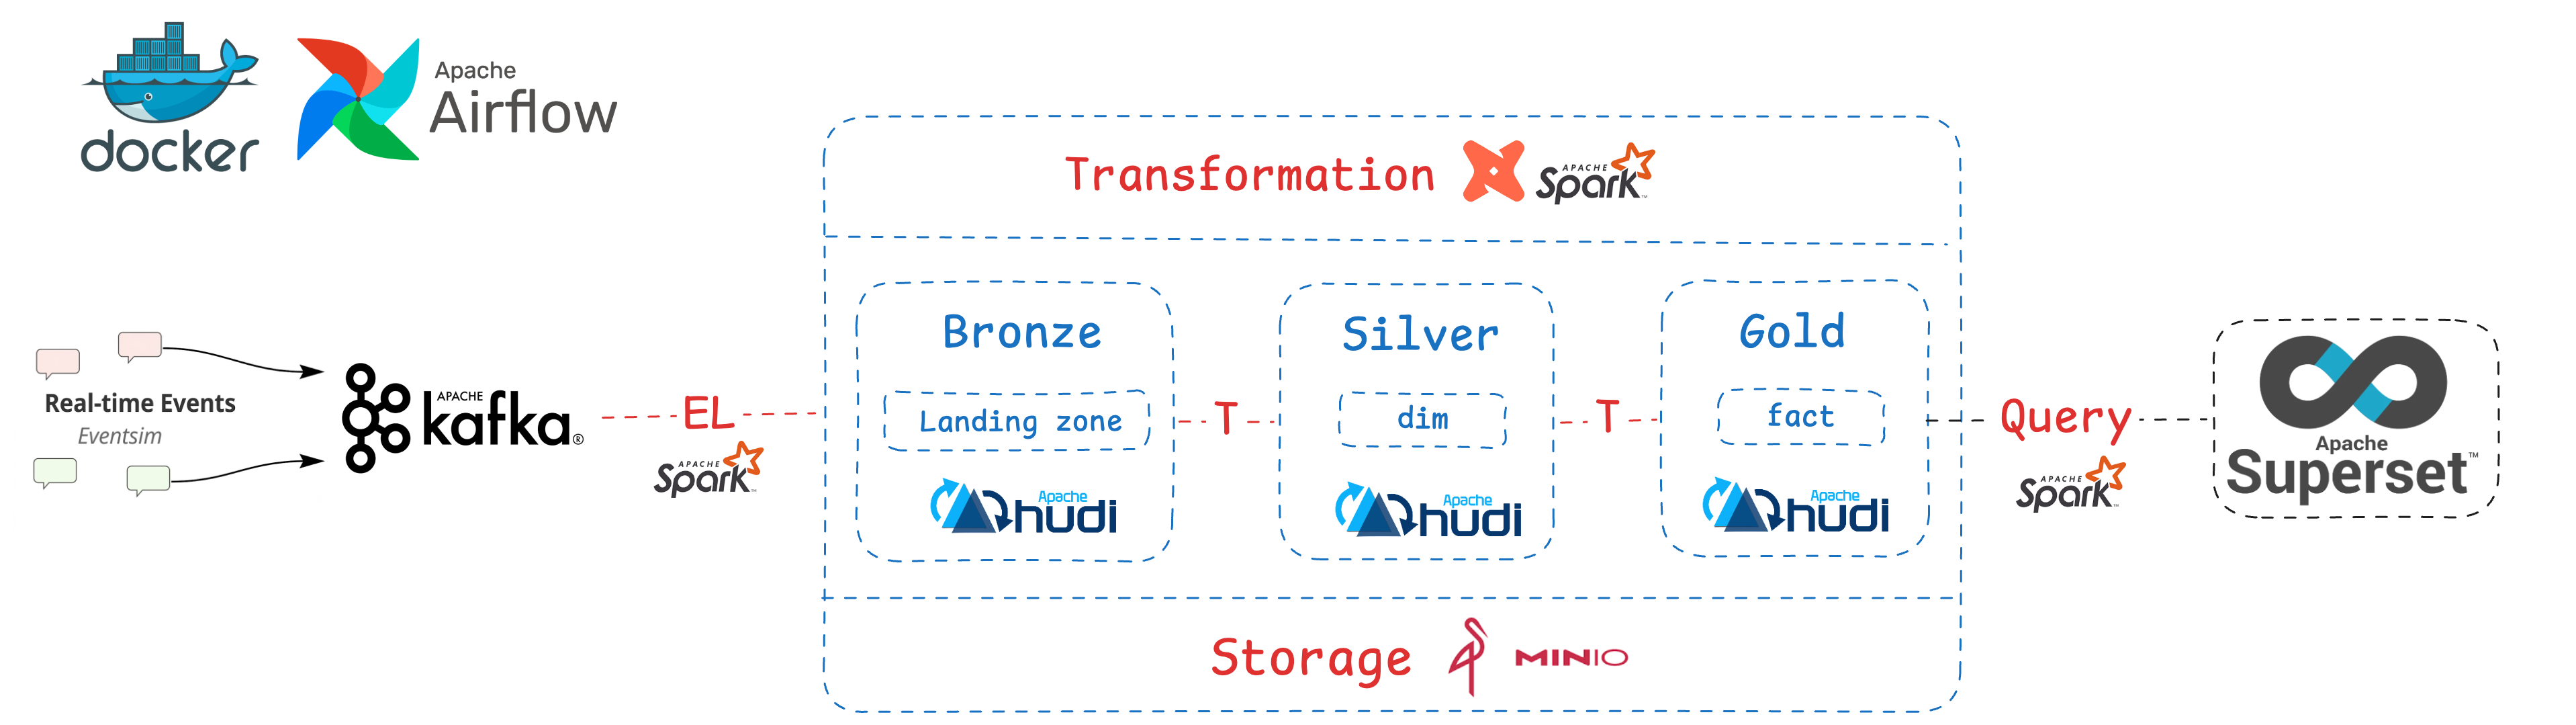
\includegraphics[width=0.8\textwidth]{overview.png}
    \caption{Streamify architecture overview.}
    \label{fig:overview}
\end{figure}

Figure~\ref{fig:overview} shows the end-to-end architecture: Eventsim generates events into a Kafka~\cite{kafka} cluster, Spark Structured Streaming~\cite{spark-structured-streaming} consumes and lands them as Hudi~\cite{hudi} bronze tables, dbt transforms the bronze layer into silver dimension tables and gold fact/wide tables on the same Spark cluster, Superset visualizes the result through the Spark Thrift Server, and Airflow schedules the dbt, dashboard-refresh and compaction jobs, alongside a Prometheus/Grafana monitoring stack.

\begin{table}[!htbp]
    \centering
    \small
    \begin{tabulary}{\textwidth}{|p{3.5cm}|p{4cm}|L|}
        \hline
        \textbf{Layer} & \textbf{Tool} & \textbf{Role} \\
        \hline
        Data simulation & Eventsim & Generates synthetic music-streaming events based on the Million Song Dataset \\
        \hline
        Message queue & Apache Kafka 4.3 (KRaft) & 2-node cluster, replication factor 2, 3 partitions per topic, no ZooKeeper \\
        \hline
        Stream processing & Spark Structured Streaming 3.5.3 & Reads Kafka, decodes/enriches events, writes bronze tables to Hudi \\
        \hline
        Table format / storage & Apache Hudi / Minio & MERGE\_ON\_READ bronze streaming tables, COPY\_ON\_WRITE silver/gold/seed tables, on MinIO/S3 via the Hadoop S3A connector \\
        \hline
        Compute cluster & Spark Standalone (1 master, 2 workers) & Shared by the streaming job and dbt (via Thrift), 4 cores total \\
        \hline
        Transformation & dbt (\texttt{dbt-spark}, \texttt{method: thrift}) & SQL-based star schema and wide-table modelling, incremental \texttt{merge} by key, submitted via the Spark Thrift Server \\
        \hline
        Orchestration & Apache Airflow 3 & Runs dbt and the Superset refresh every 30 minutes and Hudi compaction every 6 hours, one job at a time through the Thrift Server \\
        \hline
        Visualization & Apache Superset & Dashboards connected to the Spark Thrift Server \\
        \hline
        Monitoring & Prometheus, Grafana & Kafka consumer-group lag, Spark JVM/streaming metrics, per-container CPU/memory \\
        \hline
        Containerization & Docker Compose & Single-command reproducible deployment \\
        \hline
    \end{tabulary}
    \caption{Technology stack per pipeline layer.}
\end{table}

The rest of this chapter walks through the layers one by one, then the deployment. Each layer ends with a short note on why the tool was chosen (see Chapter~\ref{ch:related-work-background}).


\section{Storage Layer}
\label{sec:storage-layer}

Tables are Hudi-managed, backed by MinIO~\cite{minio} (S3-compatible) via the Hadoop S3A connector. There is no separate catalog service: each table is self-describing at its storage path (a \texttt{.hoodie/} metadata directory) and is (re-)registered into Spark's catalog idempotently at job startup. Bronze tables use the MERGE\_ON\_READ table type, so streaming writes are cheap and any delta log files are merged into columnar base files by a scheduled compaction job (Section~\ref{sec:orchestration-layer}); silver, gold, and seed tables use COPY\_ON\_WRITE, where dbt merges new rows into the existing files.

\textbf{Why Hudi, and why MOR bronze / COW silver and gold.} Hudi's self-describing \texttt{.hoodie/} metadata avoids the extra catalog or warehouse service that plain Parquet or Snowflake would require. Bronze uses MOR to keep frequent streaming appends cheap; silver and gold use COW because they are written in batches by dbt and then read repeatedly -- by downstream dbt models or by Superset. The bronze writer currently uses Hudi's \texttt{insert} operation, which adds new Parquet files and no log files, so compaction finds nothing to merge until updates or deletes reach a bronze table.

\section{Ingestion Layer}

\begin{figure}[H]
    \centering
    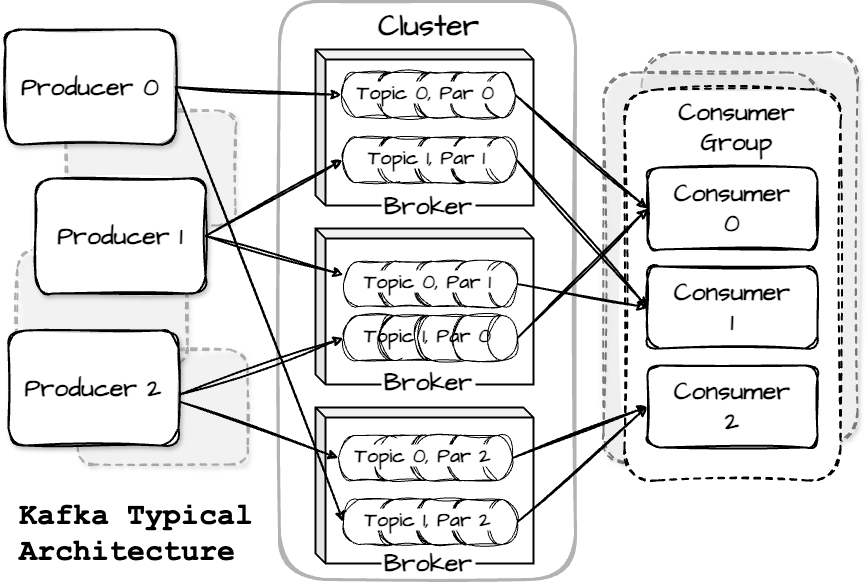
\includegraphics[width=0.4\textwidth]{4/kafka_architecture.png}
    \caption{Kafka cluster: 2 KRaft nodes, 3 partitions per topic, replication factor 2.}
    \label{fig:kafka-architecture}
\end{figure}

Eventsim simulates a real-world user base, generating page-view and song-play events that mimic activity on a music-streaming website. Apache Kafka 4.3 runs in KRaft mode (no ZooKeeper) as a 2-node cluster (\texttt{broker-1}, \texttt{broker-2}). Each of the three event topics -- \texttt{listen\_events}, \texttt{page\_view\_events}, \texttt{auth\_events} -- has 3 partitions and replication factor 2, so every partition has a replica on both brokers, as shown in Figure~\ref{fig:kafka-architecture}.

Because KRaft mode is used, each broker itself also acts as a metadata/controller node, removing the need for a separate ZooKeeper ensemble. For each topic, the 3 partitions are spread across the two brokers, and because replication factor is 2, every partition is fully replicated: one broker holds the leader replica for a given partition and the other holds the follower replica, and the two brokers swap this role across partitions so that neither broker is leader for every partition of a topic. Producers (Eventsim) and consumers (the Spark Structured Streaming job) always read from and write to the leader replica of a partition; the follower replica only pulls data from the leader to stay in sync, and takes over as leader if its broker fails. This is what gives the cluster broker-level fault tolerance despite running on just two nodes.

\section{Stream \& Batch Processing Layer}
\label{sec:proposed-cluster-setup}

\begin{figure}[H]
    \centering
    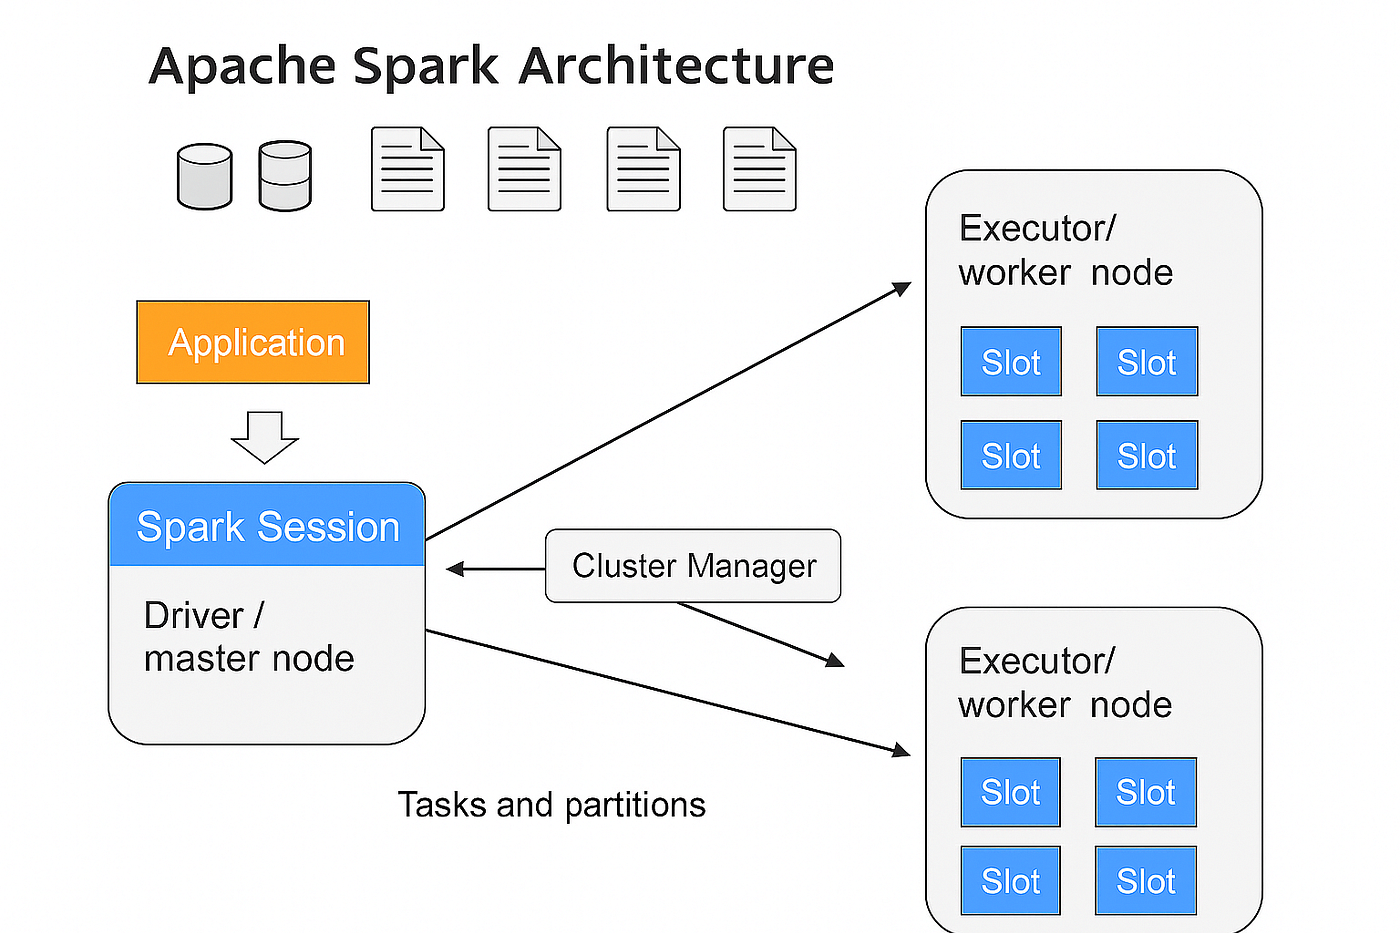
\includegraphics[width=0.4\textwidth]{4/spark_architecture.png}
    \caption{Spark cluster: driver, master, workers and executors.}
    \label{fig:spark-architecture}
\end{figure}

The whole stack runs on one machine from a single \texttt{docker-compose.yml}. Its Spark Standalone cluster, shown in Figure~\ref{fig:spark-architecture}, has 1 master and 2 workers with 2 cores / 2 GB each (4 cores in total), and runs both the streaming job and dbt's batch queries; the streaming job and the Thrift Server take 2 cores each. A \emph{driver} process plans a job and schedules its tasks; the \emph{master} tracks which workers are free and grants the driver executor slots on them; each \emph{worker} then launches one or more \emph{executor} processes that run the driver's tasks and cache data. The streaming job's driver is submitted once and keeps its executor slots for the life of the pipeline, while dbt submits short-lived batch queries through the Thrift Server on the same cluster.

\begin{figure}[H]
    \centering
    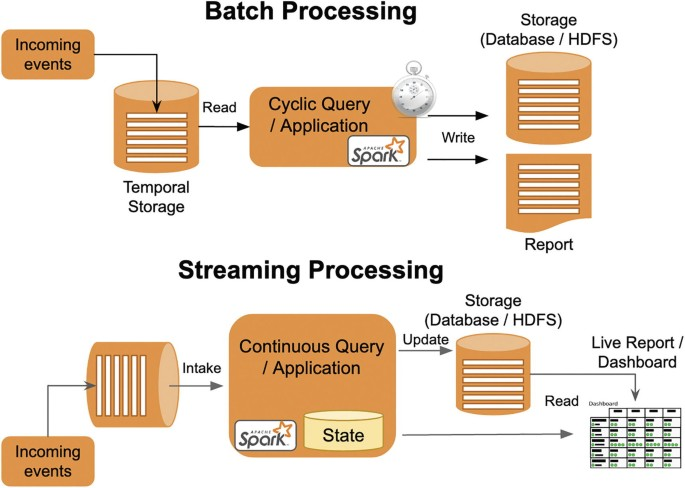
\includegraphics[width=0.4\textwidth]{4/spark_batch_streaming_processing.png}
    \caption{Micro-batch model: the stream is cut into small Spark batch jobs.}
    \label{fig:spark-micro-batch}
\end{figure}

Two layers of work share this cluster. The \emph{streaming layer} is the long-running ingestion job: it consumes all three Kafka topics, fixes latin1-mojibake on text fields, derives time columns, and appends each micro-batch to bronze Hudi tables (\texttt{staging.<topic>}). The \emph{batch layer} is everything downstream of bronze -- dbt and Superset: dbt runs on the same Spark cluster as the streaming job, reading the bronze Hudi tables and writing the silver and gold Hudi tables, and Superset connects to the Spark Thrift Server to query the gold tables for visualization.

Structured Streaming does not process events one at a time. Instead, as Figure~\ref{fig:spark-micro-batch} shows, the driver repeatedly polls the three Kafka topics for new offsets, groups the newly available records into a micro-batch, and schedules that micro-batch as a short-lived Spark job whose tasks run on the worker executors, in the same way a batch job would.

Structured Streaming resumes from a persisted checkpoint volume (\texttt{spark-checkpoints}) on restart; each micro-batch also commits its Kafka offsets to a \texttt{streamify-<topic>} consumer group purely so lag is visible in Grafana (Spark itself never depends on that commit to resume).

\section{Transformation Layer}
\label{sec:transformation-layer}

\begin{figure}[H]
    \centering
    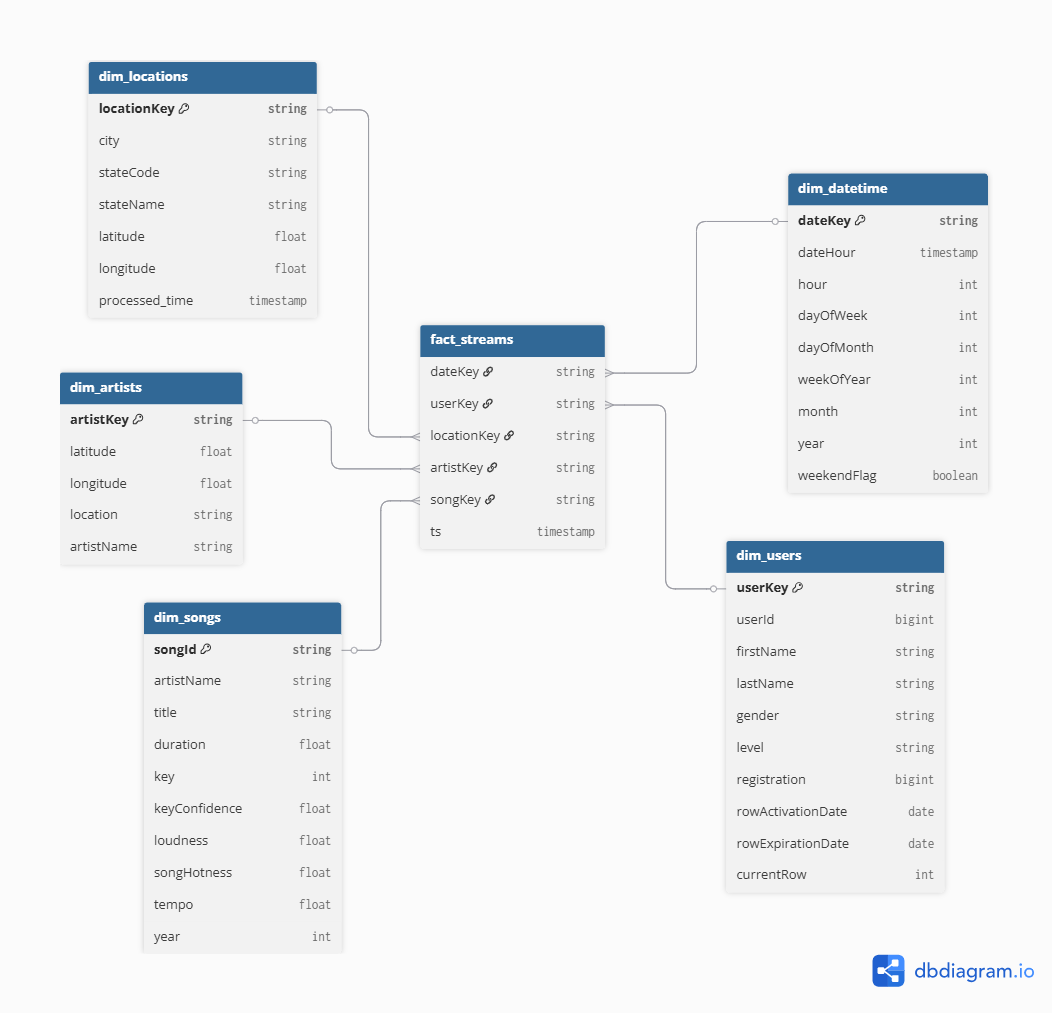
\includegraphics[width=0.35\textwidth]{star_schema.png}
    \caption{Star schema: \texttt{fact\_streams} and five dimensions.}
    \label{fig:star-schema}
\end{figure}

The transformation layer turns each bronze Hudi table into an analytical data model over two further medallion layers, silver and gold (Section~\ref{sec:core-theory}), so downstream queries never touch bronze directly:

\begin{itemize}
    \item \textbf{Silver -- dimension tables.} Five dimension tables built from bronze: \texttt{dim\_users}, \texttt{dim\_songs}, \texttt{dim\_artists}, \texttt{dim\_locations}, and \texttt{dim\_datetime}. Each cleans and conforms one entity out of the raw bronze events, independent of any one fact table.
    \item \textbf{Gold -- star schema.} The fact table \texttt{fact\_streams}, built from bronze joined against the five silver dimensions. This is the normalized, storage-efficient model (Section~\ref{sec:core-theory}).
    \item \textbf{Gold -- wide table (\texttt{wide\_streams}).} A denormalized table built by pre-joining \texttt{fact\_streams} with all five silver dimension tables, so that Superset can query a single flat table instead of performing joins at dashboard-query time.
\end{itemize}

\begin{figure}[H]
    \centering
    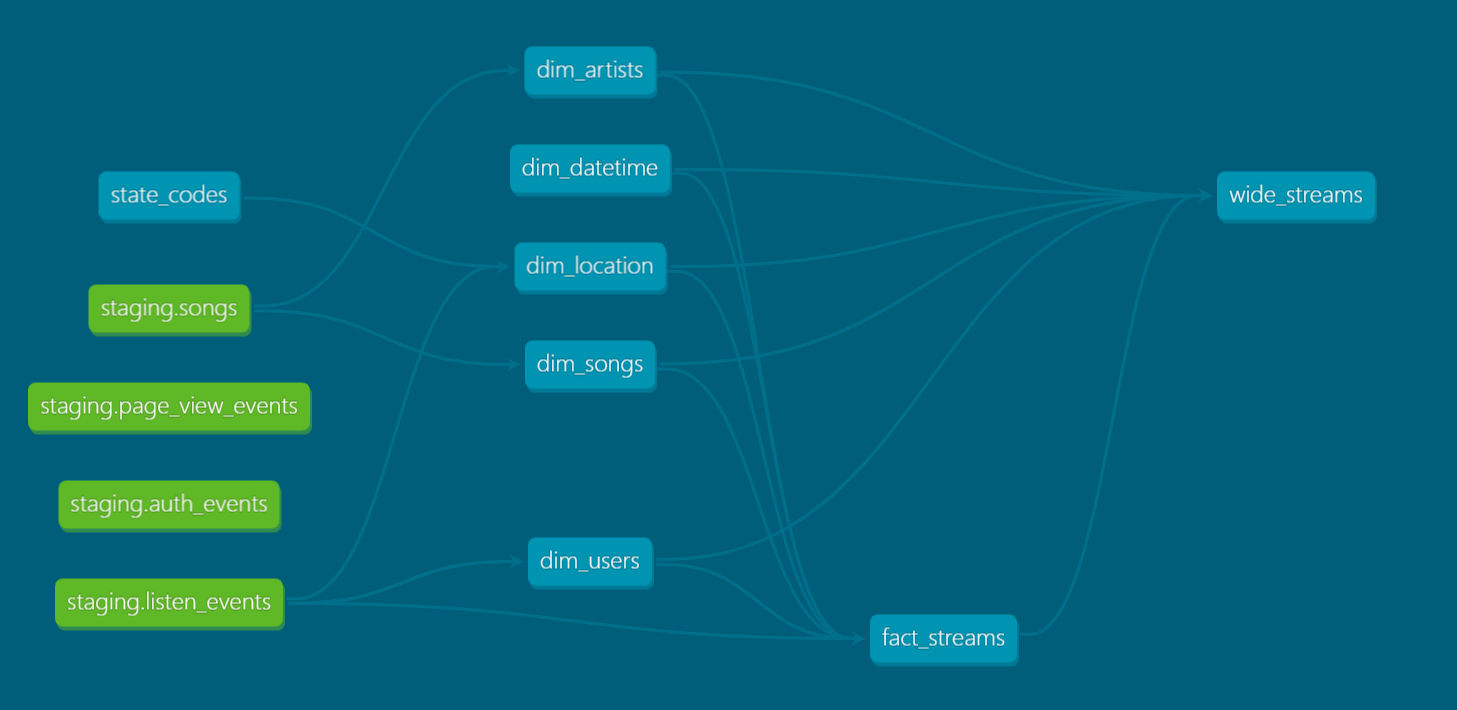
\includegraphics[width=0.35\textwidth]{dbt_graph.png}
    \caption{dbt DAG: bronze sources, star schema, \texttt{wide\_streams}.}
    \label{fig:dbt-graph}
\end{figure}

Instead of hand-written Spark jobs, dbt~\cite{dbt} generates the Spark SQL and submits it through the Spark Thrift Server (\texttt{method: thrift}), materializing every silver and gold model as a COPY\_ON\_WRITE Hudi table. The fact table, the wide table and the user and location dimensions are incremental models that \texttt{merge} new rows by a unique key; the other dimensions are rewritten per partition with \texttt{insert\_overwrite}. dbt builds a DAG of models -- declared in \texttt{dbt\_project.yml}, with each model a SQL query under \texttt{models/} -- where every model transforms one or more upstream models into a new table. Figure~\ref{fig:dbt-graph} shows the resulting DAG, with bronze sources at the bottom, the silver dimension tables next, the gold \texttt{fact\_streams} after that, and \texttt{wide\_streams} at the top.

\textbf{Why dbt, and why both a star schema and a wide table.} dbt declares model dependencies explicitly (via \texttt{ref()}/\texttt{source()}), runs built-in tests (uniqueness, not-null, referential integrity) and generates documentation from the same files, which matters for a fact table that depends on five dimensions. The star schema keeps normalization and storage efficiency, while \texttt{wide\_streams} keeps BI queries simple.

\section{Serving Layer}
\label{sec:serving-layer}

\begin{figure}[H]
    \centering
    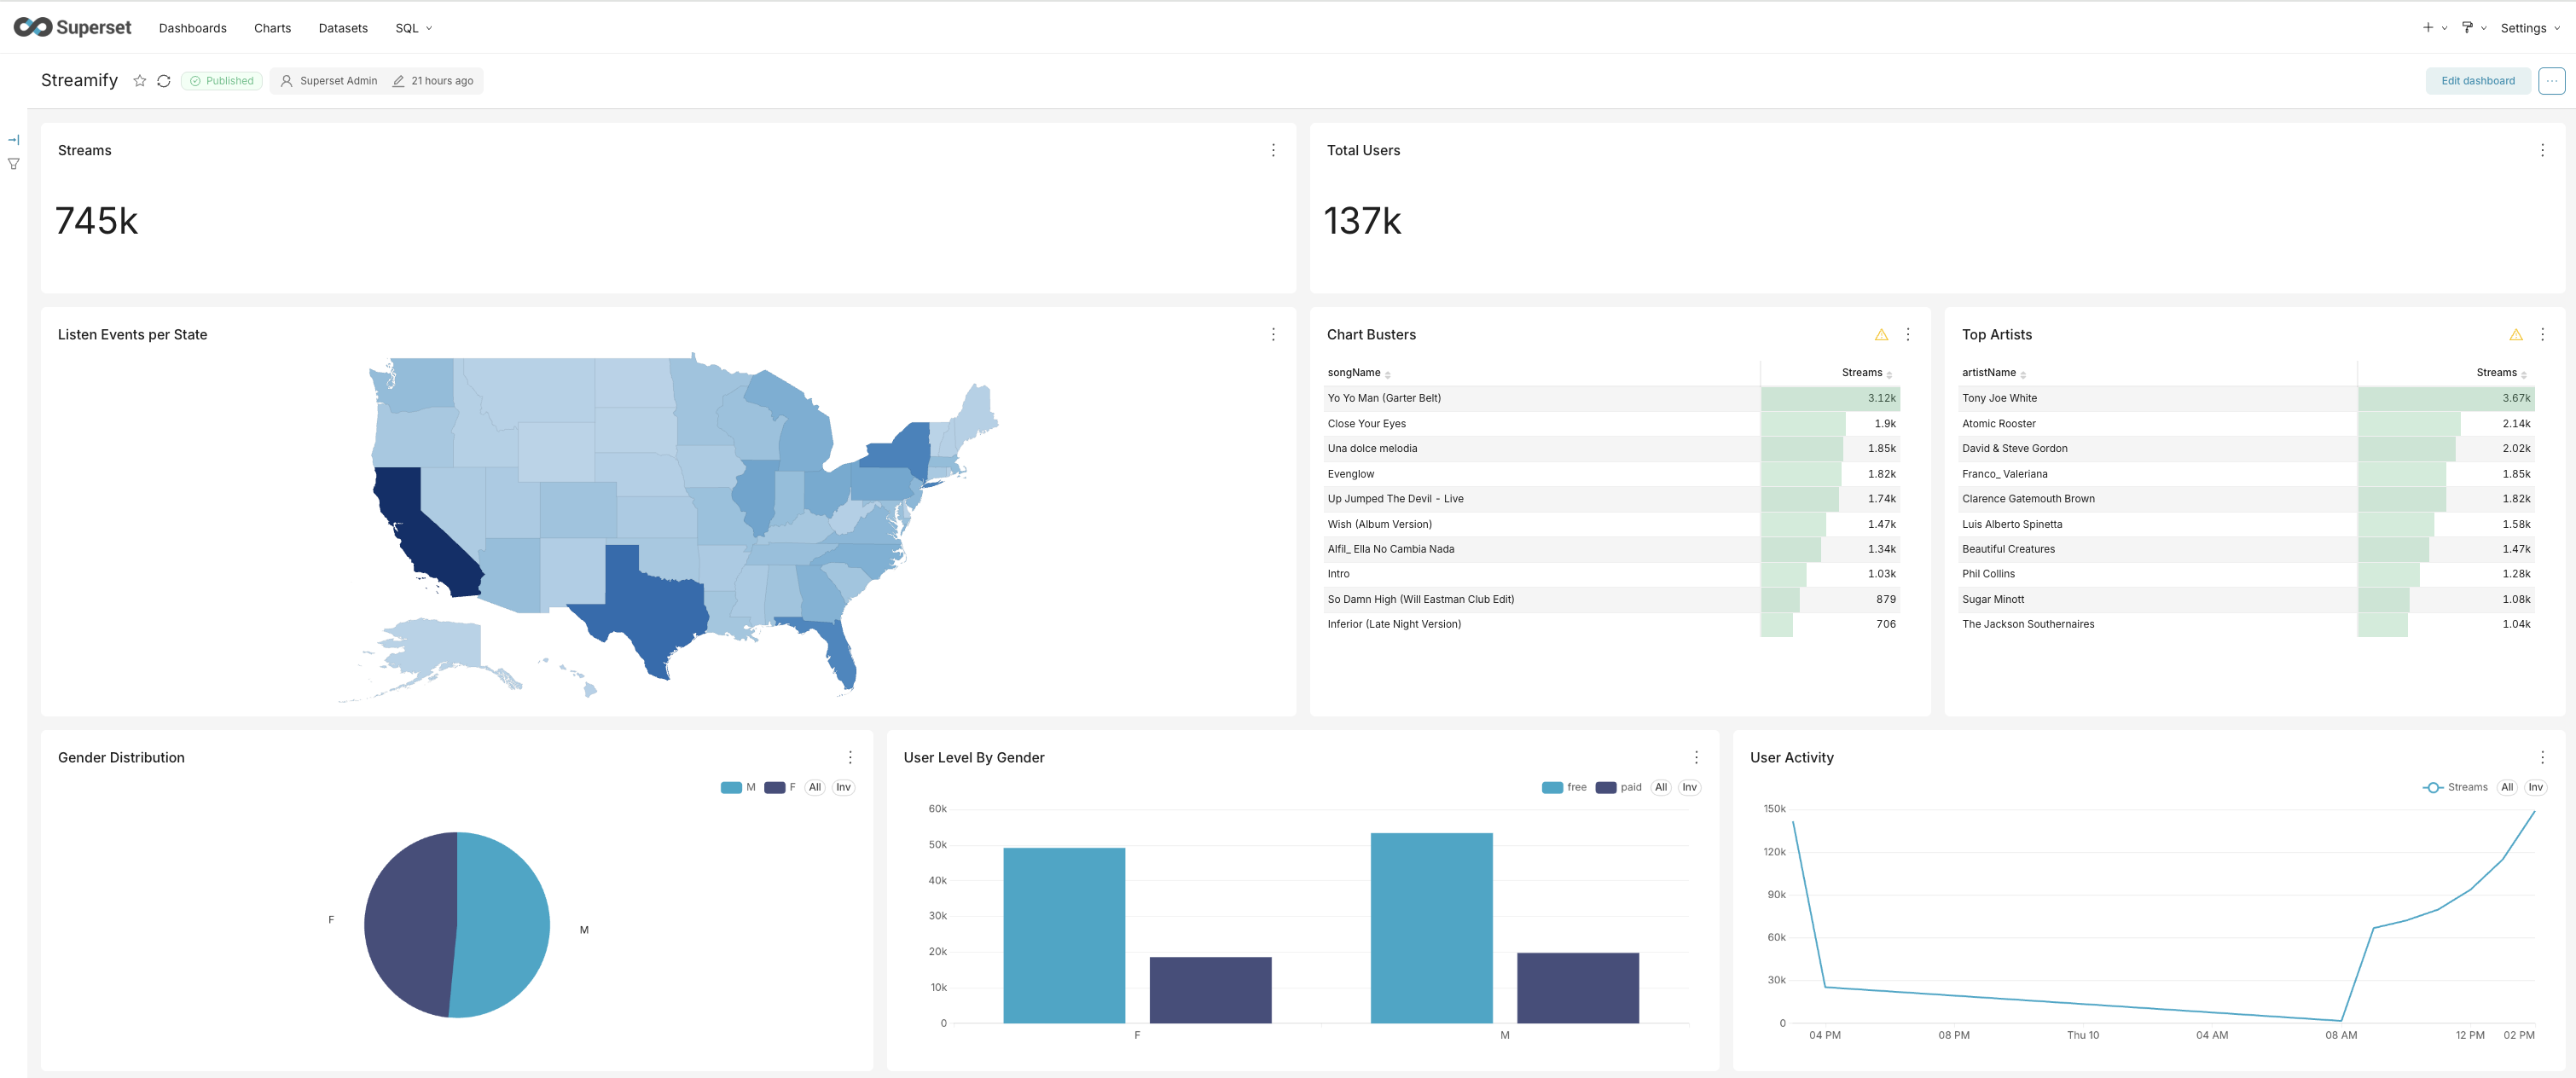
\includegraphics[width=0.65\textwidth]{dashboard.png}
    \caption{Superset dashboard on \texttt{wide\_streams}, queried via Spark Thrift Server.}
    \label{fig:results-dashboard}
\end{figure}

Apache Superset~\cite{superset} connects to the same Spark Thrift Server that dbt submits SQL through, querying the \texttt{wide\_streams} model to visualize insights through interactive dashboards (\texttt{superset/provision\_dashboard.py} provisions them via the REST API). Figure~\ref{fig:results-dashboard} shows the resulting dashboard layout.

\section{Orchestration Layer}
\label{sec:orchestration-layer}

Streaming runs all the time, but the rest of the pipeline has to be started by something: dbt must rebuild the models, the dashboard must pick up the new columns, and the Hudi tables need maintenance from time to time. At first these steps were run by hand, which is easy to forget. Apache Airflow 3 now does this. It runs as one container in standalone mode, which is enough for a single-machine demo. The DAGs are unpaused when created, so the schedules start as soon as the stack is up.

\begin{figure}[!htbp]
    \centering
    \begin{minipage}{0.49\textwidth}
        \centering
        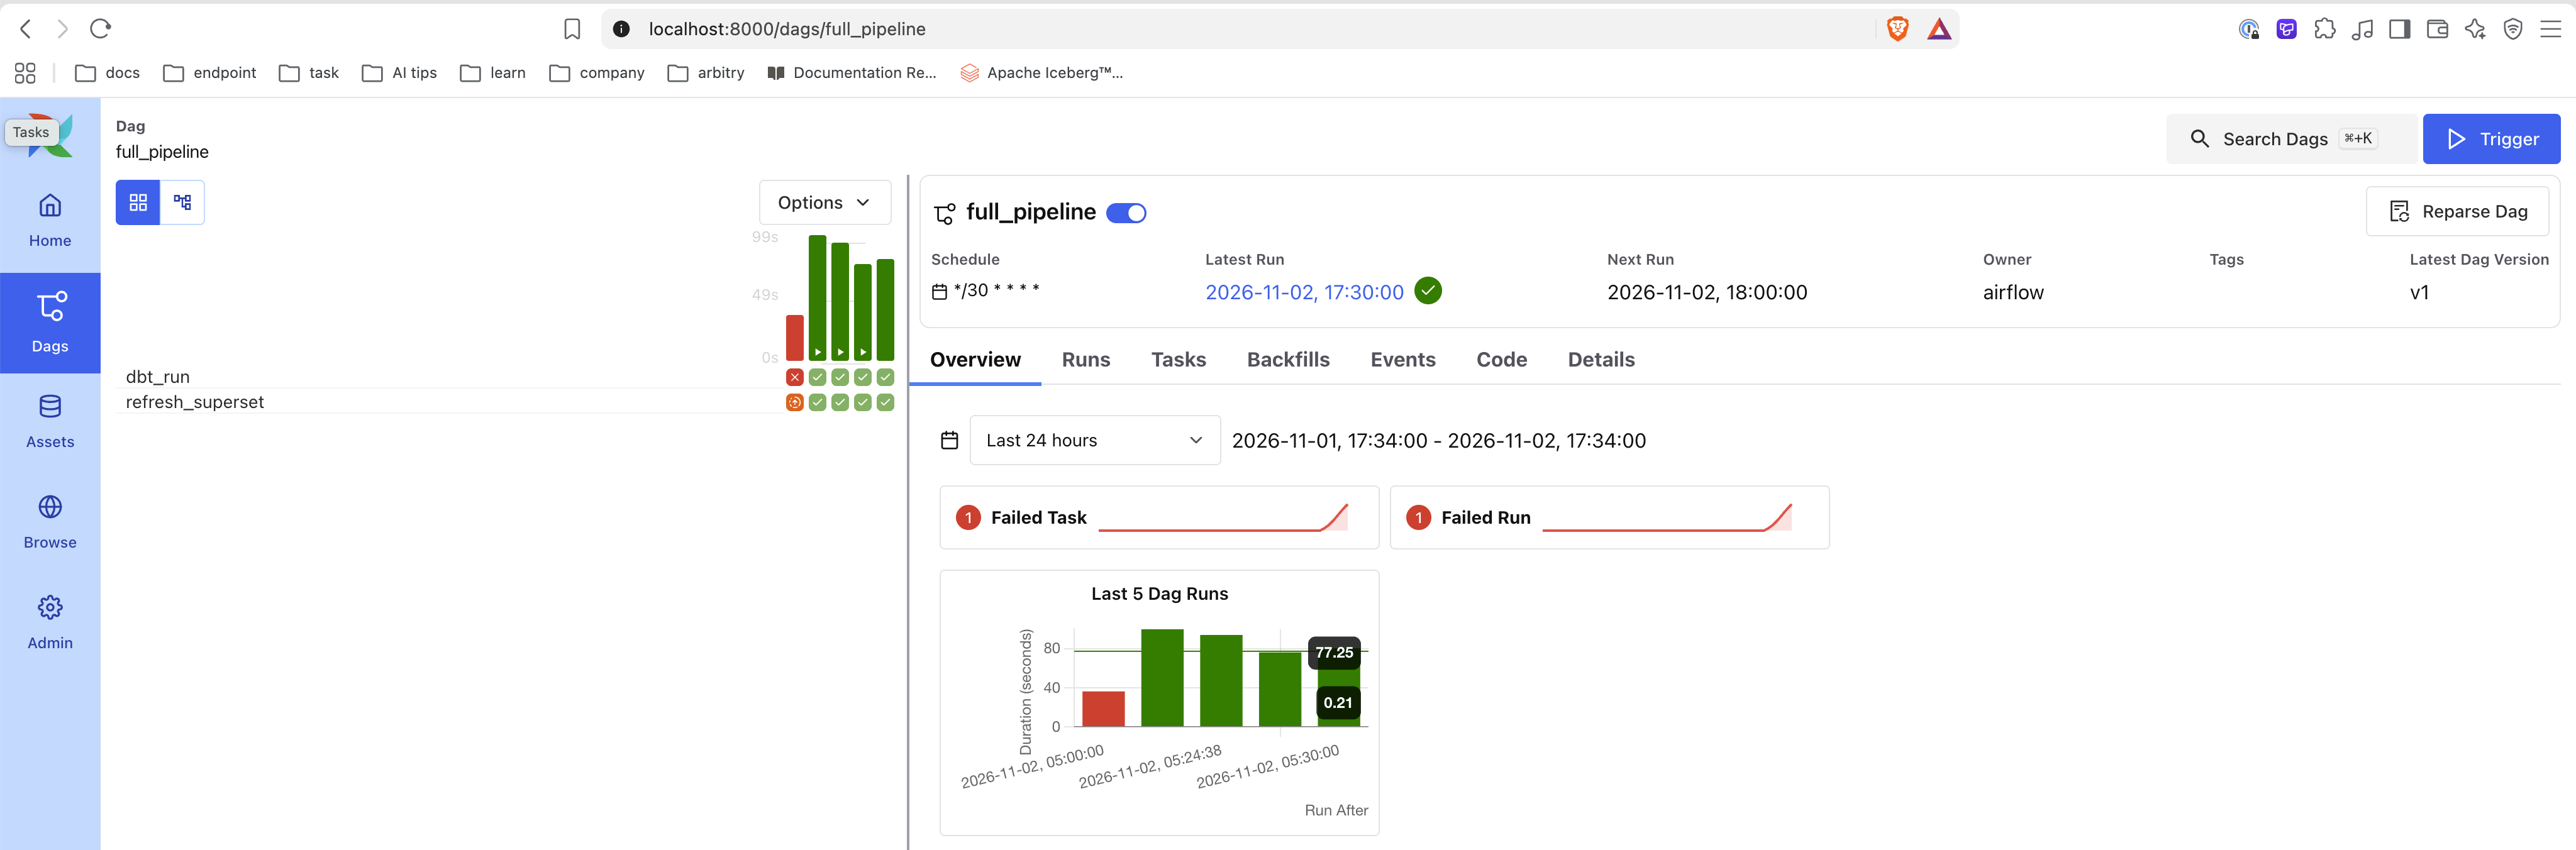
\includegraphics[width=\textwidth]{airflow_pipeline.png}
        \caption{\texttt{full\_pipeline} DAG, every 30 min. The red run failed before the seed fix.}
        \label{fig:airflow-pipeline}
    \end{minipage}\hfill
    \begin{minipage}{0.49\textwidth}
        \centering
        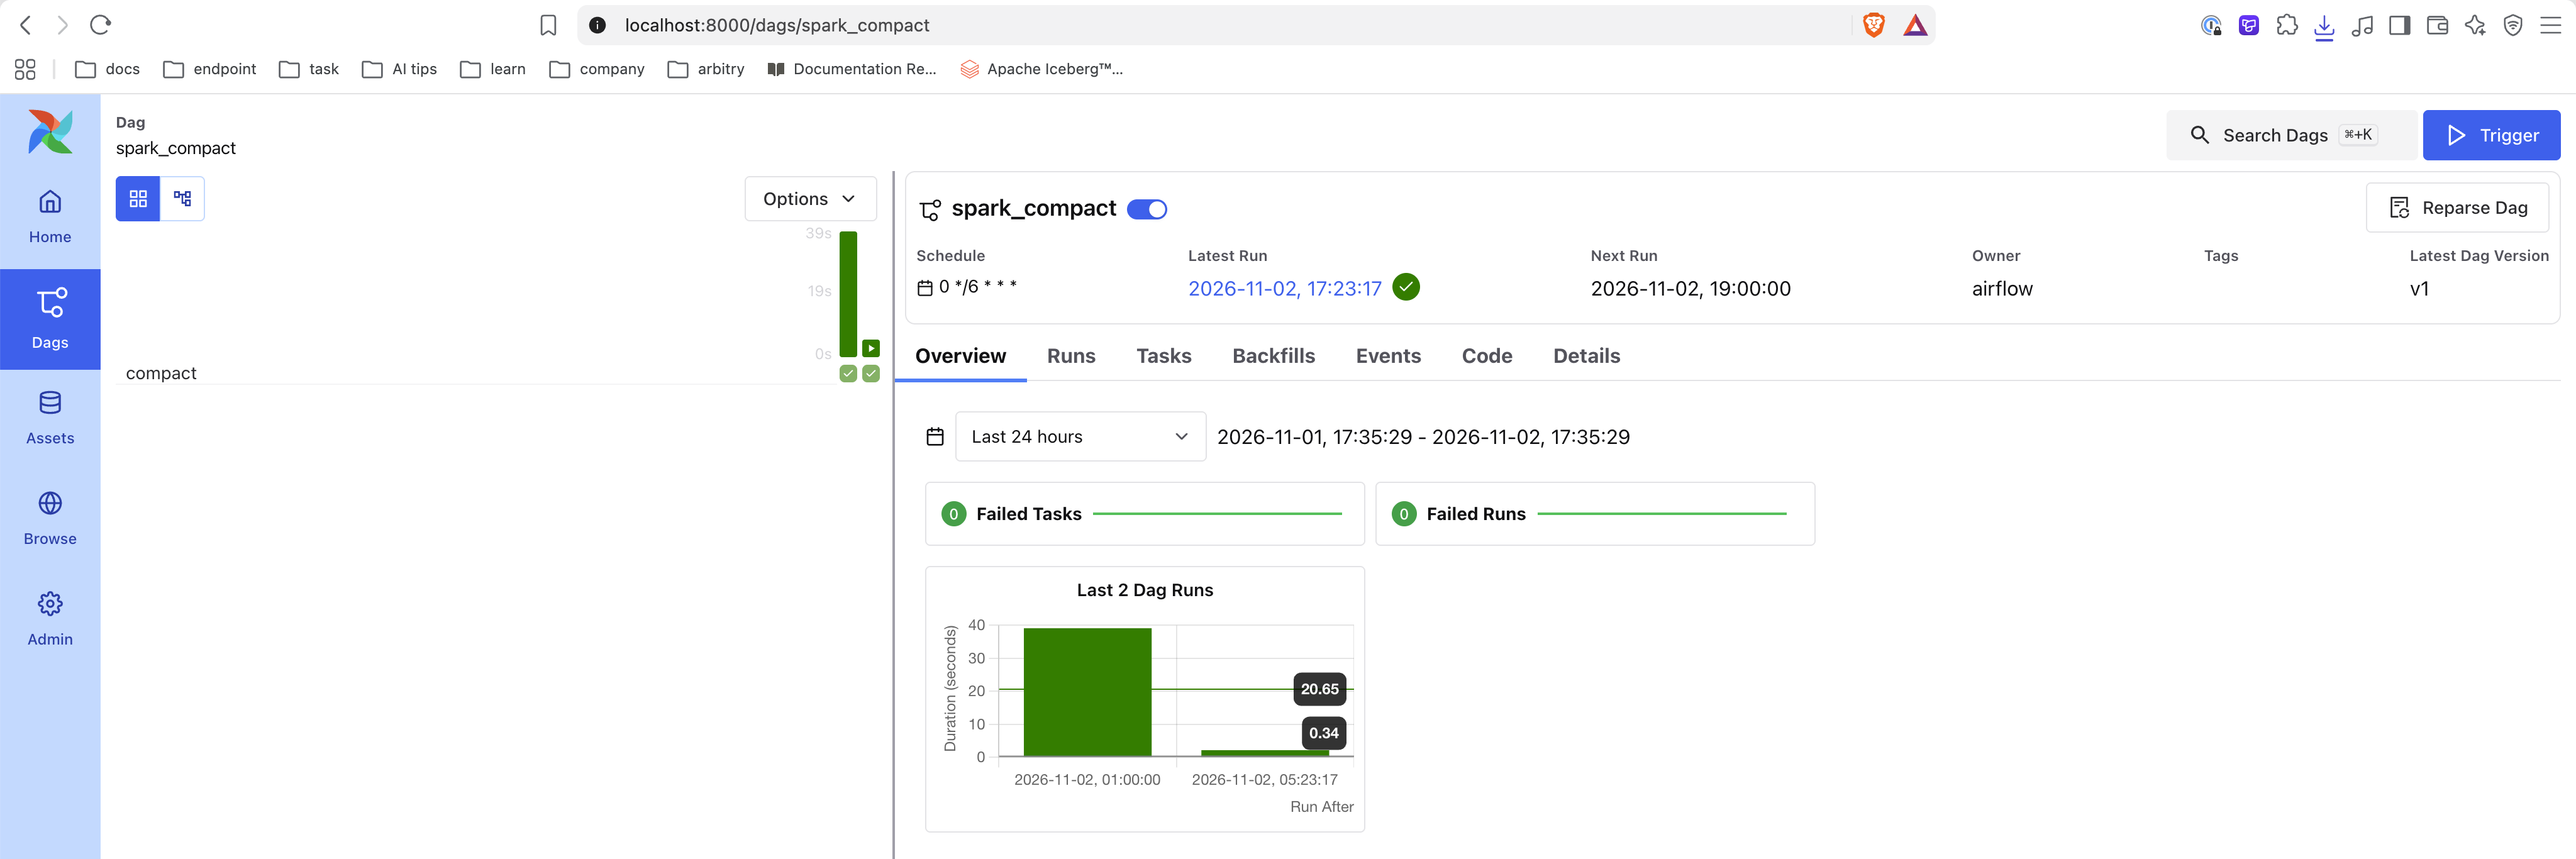
\includegraphics[width=\textwidth]{airflow_compact.png}
        \caption{\texttt{spark\_compact} DAG, every 6 h, one \texttt{compact} task.}
        \label{fig:airflow-compact}
    \end{minipage}
\end{figure}

There are three DAGs (Figures~\ref{fig:airflow-pipeline} and~\ref{fig:airflow-compact}). \texttt{full\_pipeline} runs every 30 minutes and has two tasks. The first, \texttt{dbt\_run}, loads the \texttt{state\_codes} seed and then runs all dbt models. The seed step is needed because \texttt{dbt run} does not create seed tables, and \texttt{dim\_locations} reads from one. The second task, \texttt{refresh\_superset}, first runs the dashboard provisioning script and then refreshes the dataset columns. The provisioning script is safe to repeat: it creates the dataset and dashboard only when they are missing. We added it after a fresh stack failed with ``dataset not found'', because the refresh ran before anything had created the dataset.

\texttt{spark\_compact} runs every 6 hours and calls Hudi's \texttt{run\_compaction} for each of the three bronze MOR tables. Hudi's default lock provider needs an atomic file create, which S3A does not offer, so the first runs failed with an ``unsupported scheme'' error. The job now passes an in-process lock provider in the call options. This lock only protects against other writers inside the Thrift Server, not against the streaming job, which is a separate process; a production system would need a Hive-metastore or ZooKeeper lock. Today every call returns an empty list, because the streaming writer only adds new Parquet files and never creates the log files that compaction merges (Section~\ref{sec:storage-layer}). The job is ready, but has real work only once updates or deletes reach a bronze table. The third DAG, \texttt{dbt\_adhoc}, is started by hand and shows a small form where the user picks the dbt command, the model selection and whether to do a full refresh, so one-off runs need no code change.

All three DAGs send SQL to the same Spark Thrift Server instead of starting their own Spark applications, since the cluster has no free core for another one (Section~\ref{sec:proposed-cluster-setup}). Two of them at once would compete for the Thrift Server's 2 cores, so they share an Airflow pool called \texttt{thrift\_pool} with a single slot and take turns. dbt itself is installed in its own virtual environment inside the Airflow image, with its packages fetched at image build time.

\section{Monitoring Layer}
\label{sec:monitoring-layer}

\begin{figure}[H]
    \centering
    \begin{minipage}{0.49\textwidth}
        \centering
        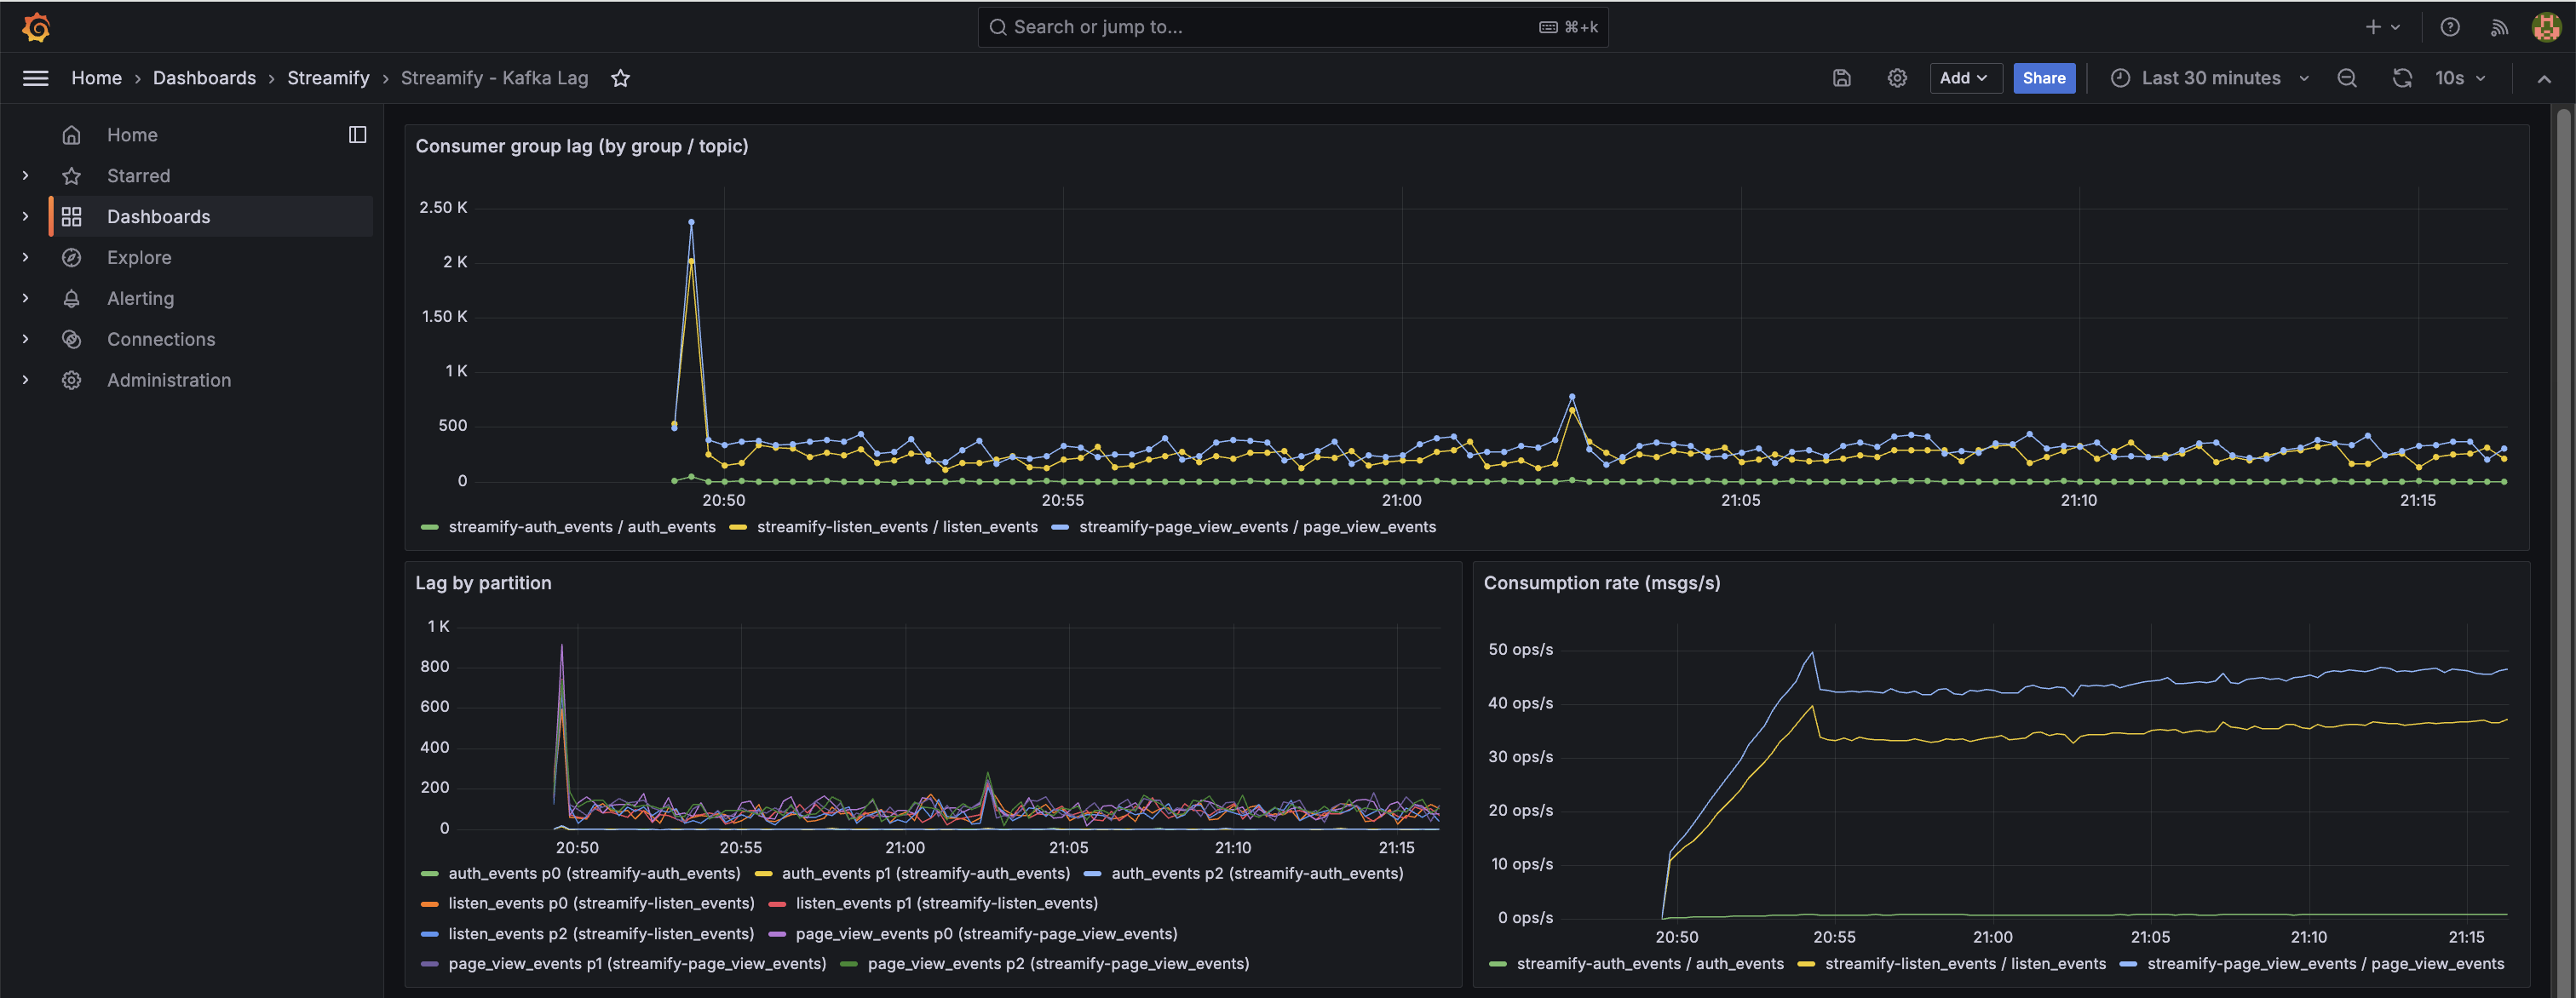
\includegraphics[width=\textwidth]{grafana_kafka.png}
        \caption{Grafana Kafka dashboard: consumer lag and rate per topic.}
        \label{fig:grafana-kafka}
    \end{minipage}\hfill
    \begin{minipage}{0.49\textwidth}
        \centering
        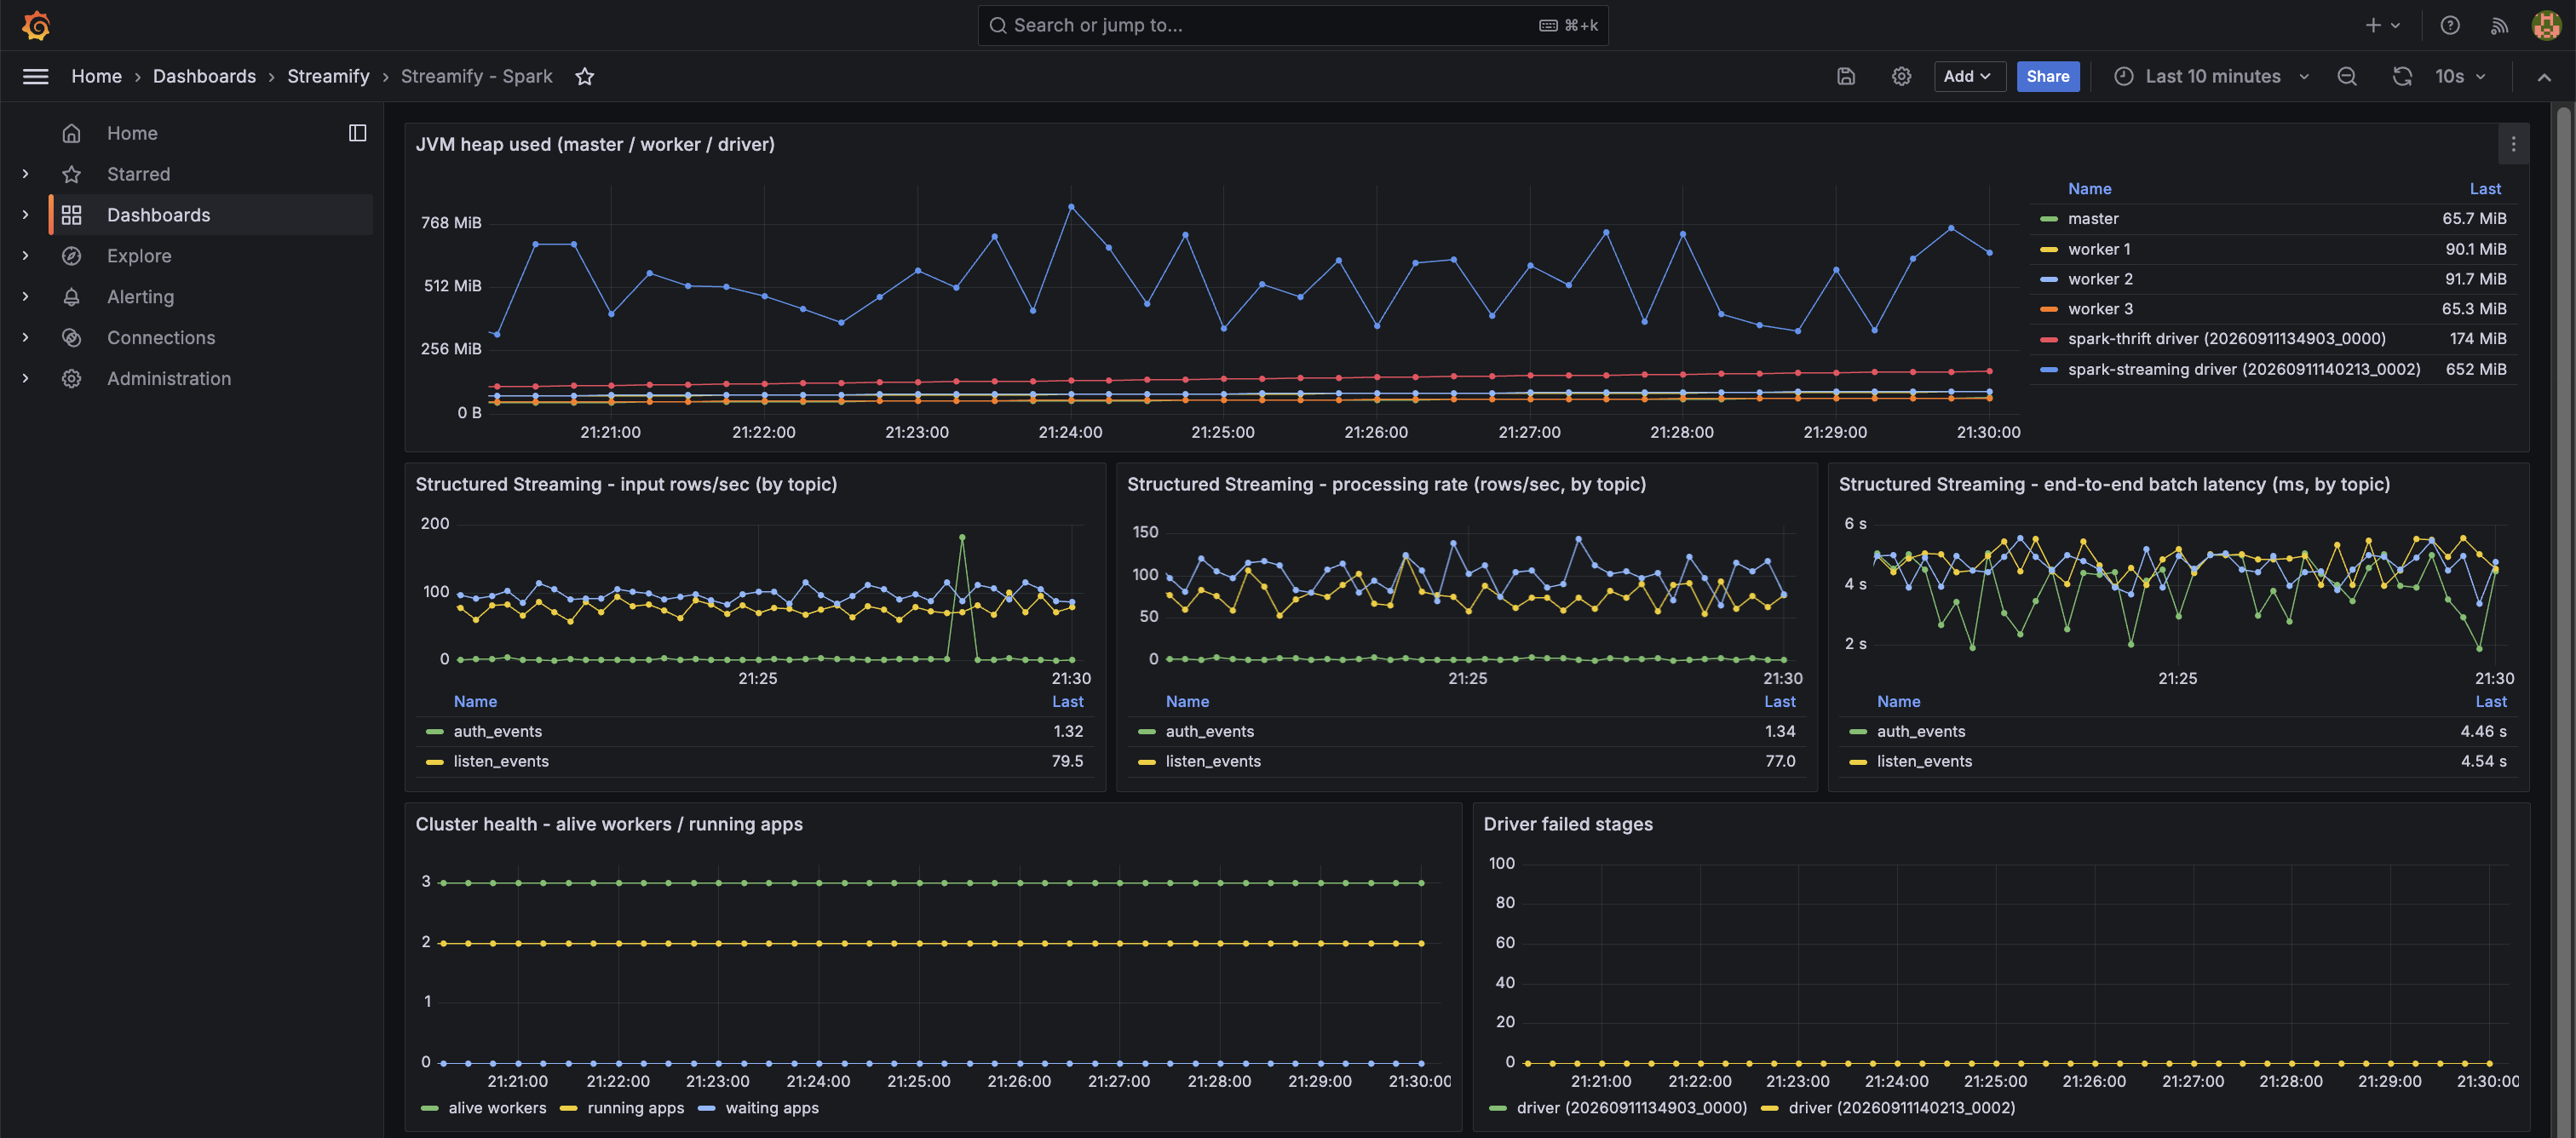
\includegraphics[width=\textwidth]{grafana_spark.png}
        \caption{Grafana Spark dashboard: job metrics, JVM heap, container CPU/memory.}
        \label{fig:grafana-spark}
    \end{minipage}
\end{figure}

Three exporters feed one Prometheus instance: kafka-exporter (consumer-group lag per partition), Spark's metrics endpoint (streaming/batch counters, JVM heap) and cAdvisor (per-container CPU and memory). Grafana renders them in Figures~\ref{fig:grafana-kafka} and~\ref{fig:grafana-spark}.
